%%%%%%%%%%%%%%%%%%%%%%%%%%%%%%%%%%%%%%%%%
% Wireless BERA - Forschungspraxis report
% Based on the MFE report template (Makoto Technical Report, LaTeXTemplates.com,
% CC BY-NC-SA 4.0).
%
%!TEX program = xelatex
% Build: xelatex report && bibtex report && xelatex report && xelatex report
% Figures: python3 ../measurements/tools/report_figures.py
%%%%%%%%%%%%%%%%%%%%%%%%%%%%%%%%%%%%%%%%%

\documentclass[
	a4paper,english
]{MFETechnicalReport}

\sisetup{
  locale = UK,
  separate-uncertainty,
  range-units = single,
  list-units = single,
  per-mode = reciprocal,
  multi-part-units = single,
  range-phrase = {\text{~to~}},
  input-symbols = e,
  parse-numbers = true
  }

\selectlanguage{english}
\addbibresource{report.bib}

\reporttitle{Development of a Portable, Ultra-Low-Noise Biosignal Acquisition System for Brainstem Evoked Response Audiometry}
\reportsubtitle{Forschungspraxis (Master) -- Technical Report}
\reportauthors{Nathan Scheufele\\\smallskip
	Supervisor and examiner: Bernhard Gleich\\
	Munich Institute of Biomedical Engineering, Technische Universität München}
\reportdate{October 2026}
\leftheadercontent{Wireless BERA -- Forschungspraxis Report}
\rightheadercontent{
\includegraphics[width=2cm]{logos/tum.pdf}}

\begin{document}
	%---------------------------------------------------------------------------------
	%	TITLE
	%---------------------------------------------------------------------------------
	\thispagestyle{empty}
	\vspace*{-0.075\textheight}
	\hfill
\includegraphics[width=2cm]{logos/tum.pdf}
	\vspace{0.03\textheight}

	{\large\raggedright\reportdate\par}
	\vspace{0.01\textheight}
	{\fontsize{24pt}{28pt}\selectfont\raggedright\textbf{\reporttitle}\par}
	\vspace{0.025\textheight}
	{\Large\raggedright\textit{\textbf{\reportsubtitle}}\par}
	\vspace{0.03\textheight}
	{\large\raggedright\reportauthors\par}
	\vspace{0.035\textheight}

	{\centering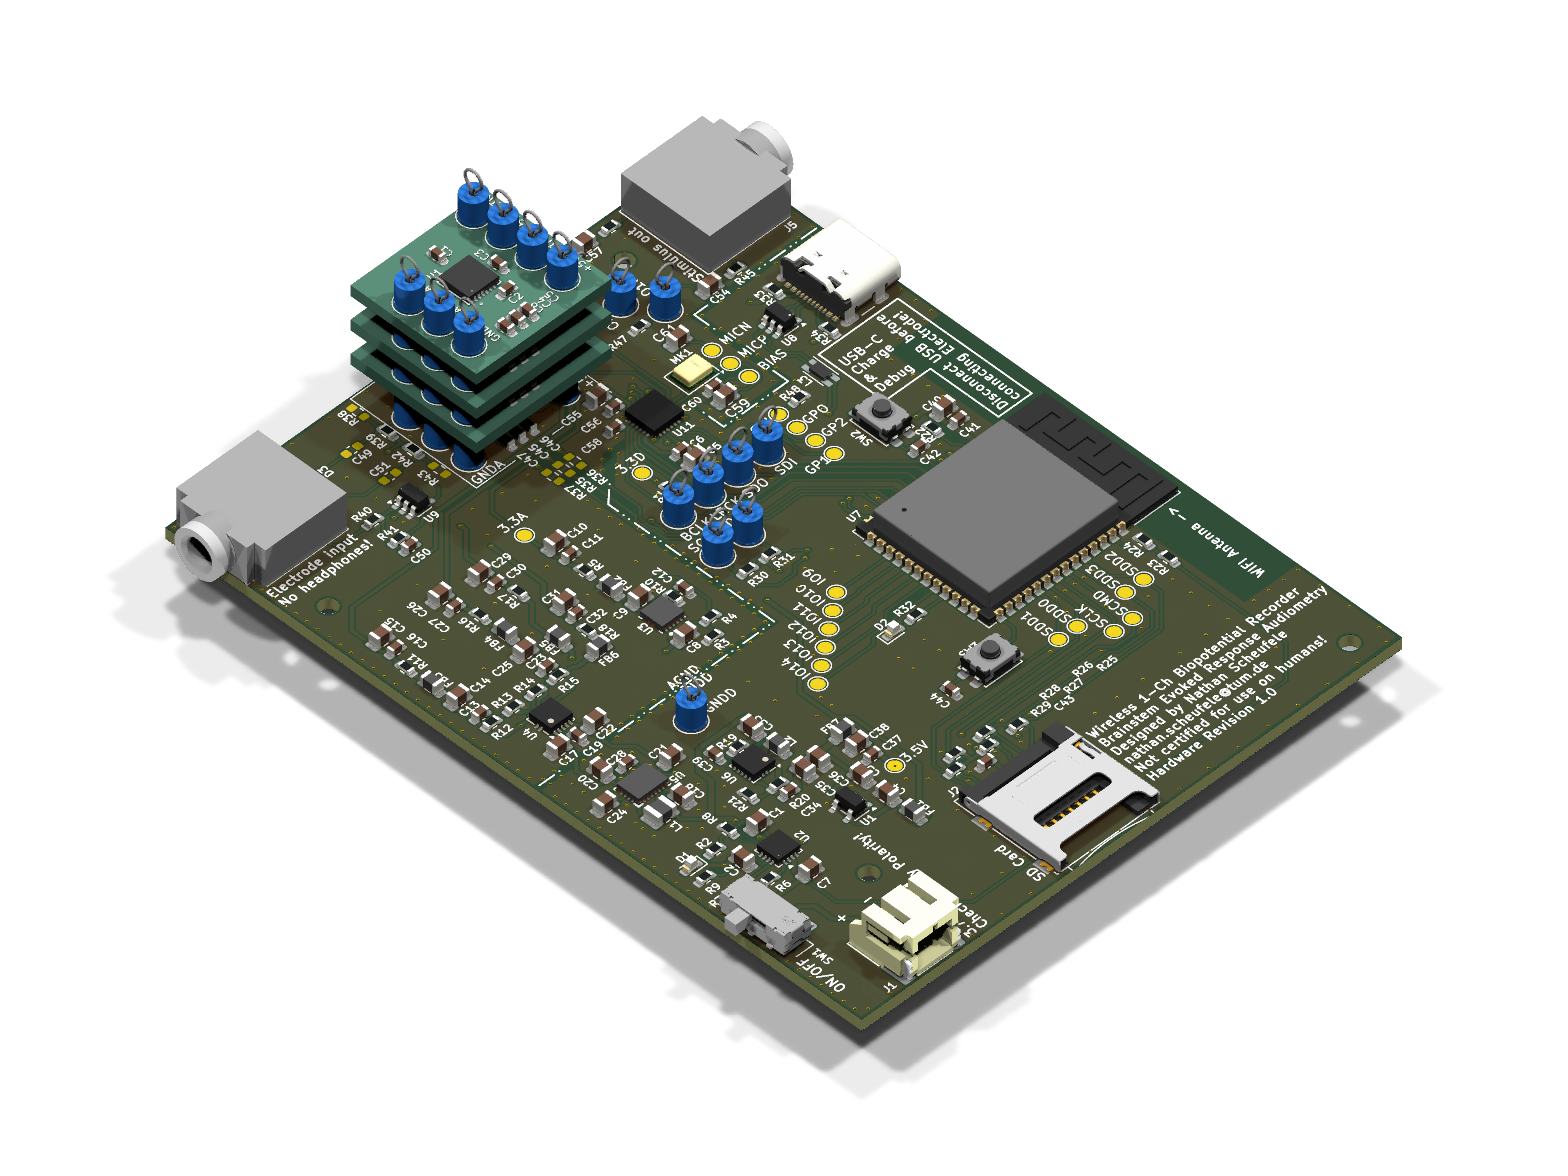
\includegraphics[width=0.72\linewidth,height=0.27\textheight,keepaspectratio,trim=150 120 150 100,clip]{figures/render_stacked_assembly.png}\par}

	\vfill
	\paragraph{Abstract}
	\emph{Wireless BERA} is a battery-powered, single-channel biopotential recorder for auditory brainstem response (ABR) audiometry that is operated from a web browser over Wi-Fi. One audio codec (TAC5212) digitises the amplified electrode signal and at the same time generates the acoustic stimulus, so stimulus and acquisition share one sample clock. In this Forschungspraxis the board was designed, manufactured as a 4-layer PCB, hand-assembled, brought up and given its firmware. It was then validated in vivo: a chest ECG agrees beat by beat with an Apple Watch (RR difference \SI{0.2 \pm 1.8}{\milli\second}), the driven right leg lowers mains pickup by \SIrange{10}{18}{\decibel}, and a click-evoked brainstem response with a wave-V candidate at \SI{6.1}{\milli\second} was recorded from the author ($p = 0.001$, permutation test), absent in an earbud-out control.

	\newpage
	\begin{multicols}{2}
		\tableofcontents

%-------------------------------------------------------------------------------------
\section{Motivation and Goals}

Brainstem evoked response audiometry records the potentials that the auditory nerve and brainstem produce within about \SI{10}{\milli\second} after an acoustic click. Wave~V, the most robust peak, is a few hundred nanovolts large and sits on microvolts of EEG, muscle activity and mains interference. It only becomes visible after averaging thousands of stimulus-locked sweeps~\cite{Hall:2007abr,Picton:2011aep}. Clinical systems are bulky, mains-connected and expensive.

The aim of this work was a compact, battery-powered alternative with
\begin{itemize}
	\item a low-noise differential front end with programmable gain,
	\item active common-mode suppression by a driven right leg (DRL)~\cite{Winter:1983drl},
	\item an acoustic stimulus output on the same clock as the acquisition,
	\item battery operation, isolated from mains while recording,
	\item wireless data transfer and operation from any browser.
\end{itemize}
The emphasis was on the hardware; the firmware was written to bring the board up and to make first measurements possible.

%-------------------------------------------------------------------------------------
\section{System Overview}

The signal paths of the board (Figure~\ref{fig:board}) are:
\begin{itemize}
	\item \textbf{Biopotential:} electrode connector J6 $\rightarrow$ LTC6373 instrumentation amplifier $\rightarrow$ TAC5212 ADC channel~2,
	\item \textbf{Sound:} microphone $\rightarrow$ ADC channel~1,
	\item \textbf{Stimulus:} TAC5212 DAC $\rightarrow$ connector J11 (insert earphone),
	\item \textbf{Common mode:} OPA376 DRL driver $\rightarrow$ third electrode,
	\item \textbf{Data:} I\textsuperscript{2}S $\rightarrow$ ESP32-S3 $\rightarrow$ Wi-Fi $\rightarrow$ browser.
\end{itemize}
Because ADC and DAC run on the same bit clock, every click falls on a fixed sample of the recording. This is the prerequisite for stimulus-synchronous averaging and was used directly in the ABR measurements (Section~\ref{sec:abr}).

\begin{figure}[H]
	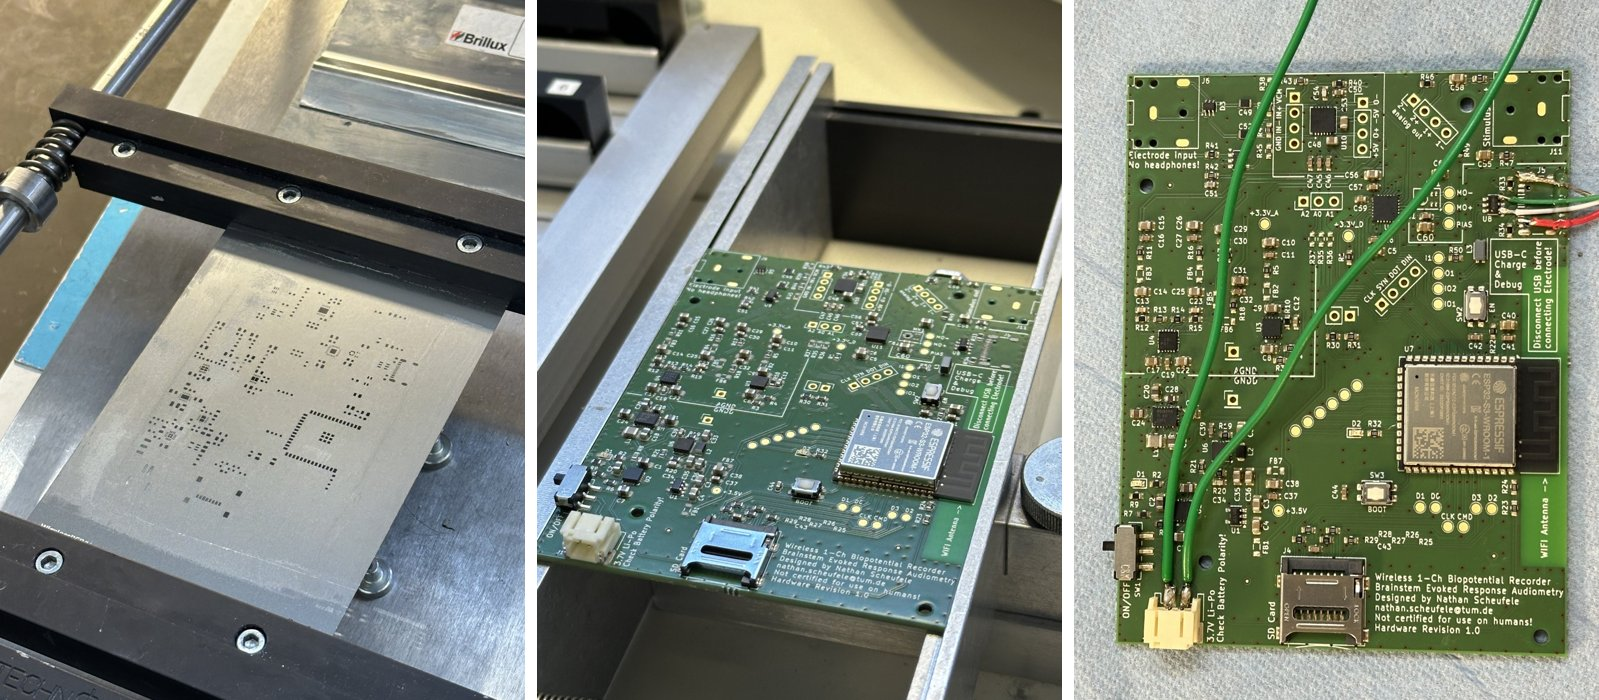
\includegraphics[width=\linewidth]{figures/fig_assembly.jpg}
	\caption{Assembly of v1.0 by hand: stencil printing of solder paste, placed components before reflow, and the assembled board with the battery leads.}
	\label{fig:board}
\end{figure}

%-------------------------------------------------------------------------------------
\section{Hardware Design}

\subsection{Analog Front End}

\paragraph{Instrumentation amplifier.} The LTC6373~\cite{ADI:LTC6373} is a fully differential instrumentation amplifier with pin-selectable gains from 0.25 to 16. It runs from clean $\pm\SI{5}{\volt}$ rails; three ESP32 GPIOs select the gain. Its output common mode is set to
\begin{equation}
	V_\text{OCM} = \SI{3.3}{\volt}\cdot\frac{\SI{10}{\kilo\ohm}}{\SI{14.99}{\kilo\ohm}} \approx \SI{2.20}{\volt},
\end{equation}
so that the output can drive the codec directly. The electrodes are AC-coupled (C49/C52) and biased through \SI{1}{\mega\ohm} to the DRL reference.

\paragraph{ADC and DAC.} The TAC5212~\cite{TI:TAC5212} samples both channels with 24-bit resolution at \SIrange{8}{96}{\kilo\hertz} and has a two-channel DAC. Full scale is \SI{2}{\volt}\,rms; at gain~16 one 16-bit step of the data stream corresponds to \SI{5.4}{\micro\volt} at the electrodes.

\paragraph{Driven right leg.} An OPA376 senses the input common mode and drives it back, inverted, into the third electrode through \SI{110}{\kilo\ohm}, which limits the current to below \SI{50}{\micro\ampere}.

\paragraph{Stimulus output.} Both DAC outputs are used single-ended, AC-coupled through \SI{22}{\micro\farad} and \SI{10}{\ohm} into a \SI{3.5}{\milli\metre} jack for insert earphones.

\subsection{Power Supply}

A single Li-ion cell is charged from USB-C by a BQ24074 with power-path management (Figure~\ref{fig:power}). A TPS63000 buck-boost supplies \SI{3.5}{\volt} for the ESP32-S3 and the microSD card. A TPS65132 charge pump generates $\pm\SI{5.4}{\volt}$, from which the TPS7A39 dual LDO~\cite{TI:TPS7A39} derives the $\pm\SI{5}{\volt}$ analog rails. The codec has its own ultra-low-noise \SI{3.3}{\volt} analog (TPS7A94) and digital (TPS7A2033) regulators. All analog rails are fed in a star through ferrite-bead LC filters. Recordings are meant to be made on battery only, which the silkscreen states next to the USB connector.

\begin{figure*}
	\centering
	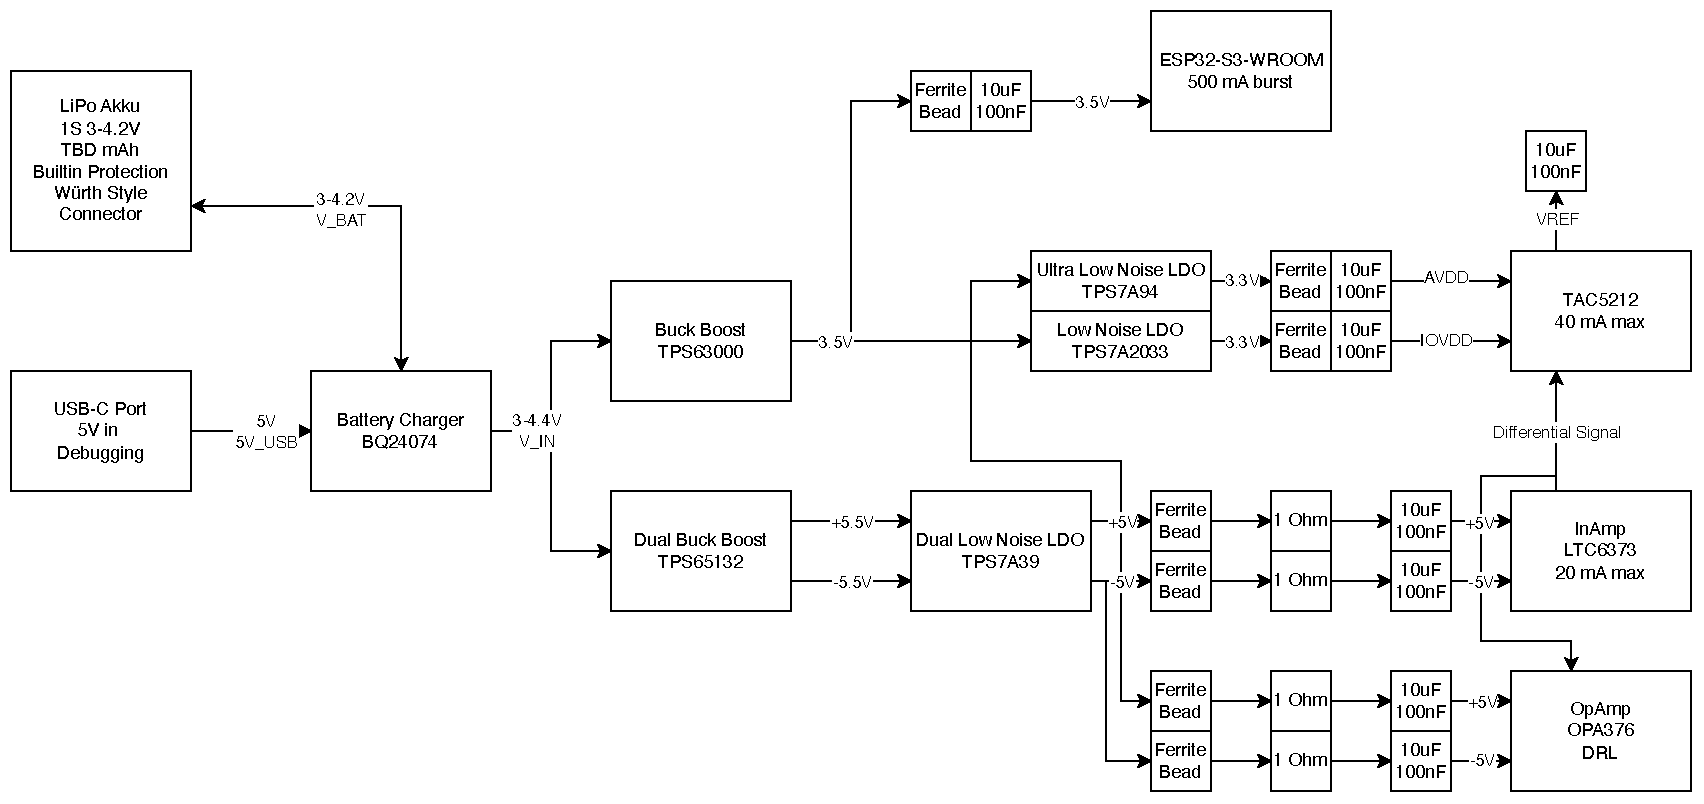
\includegraphics[width=0.92\linewidth]{figures/power_architecture.pdf}
	\caption{Power architecture of Wireless BERA v1.0.}
	\label{fig:power}
\end{figure*}

\subsection{Digital Section and PCB}

An ESP32-S3-WROOM-1-N16R8~\cite{Espressif:S3WROOM1} (\SI{16}{\mega\byte} flash, \SI{8}{\mega\byte} PSRAM) provides Wi-Fi, USB and a microSD slot. It is the I\textsuperscript{2}S clock master; the codec locks its PLL to the bit clock. The board is a 4-layer KiCad design manufactured by Aisler, with separate analog and digital grounds joined at one point and the front end placed next to the electrode connector, away from the radio and the switching regulators.

A plug-in daughterboard carries a further LTC6373 at gain~16; several can be stacked (title page) so that their uncorrelated noise averages down by about $\sqrt{n}$.

The analog design was simulated in LTspice before layout: frequency response, input-referred noise, the transient response to a modelled ABR train, and the stability of the DRL loop.

%-------------------------------------------------------------------------------------
\section{Manufacture and Bring-up}

The PCB was assembled by hand with a stencil and reflow (Figure~\ref{fig:board}). All rails came up as designed (codec AVDD \SI{3.31}{\volt}, charge pump $\pm\SI{5.4}{\volt}$), the codec and the charge pump answer on I\textsuperscript{2}C, and the codec PLL locks at all sample rates from 8 to \SI{96}{\kilo\hertz}.

Two deviations from the schematic remain on the prototype. The gain-select resistors R35--R37 are not fitted, so the amplifier runs at its default gain of~16, which is the gain intended for ABR anyway. The MEMS microphone is not fitted either; instead the electret microphone of a 4-pole earbud headset was wired to the microphone input, and its left earbud to DAC channel~2 as the stimulus transducer.

%-------------------------------------------------------------------------------------
\section{Firmware}

The ESP-IDF firmware brings the board up in a fixed order (I\textsuperscript{2}S clock before codec configuration) and serves a single web page as the complete user interface, so no software has to be installed. It provides
\begin{itemize}
	\item acquisition at \SIrange{8}{96}{\kilo\hertz}, decimated and streamed over a WebSocket, with a sequence number and the absolute frame index in every packet,
	\item on-device RMS, peak, DC and clipping meters,
	\item a stimulus generator (click, tone burst, chirp, sine, noise) with selectable rate, width and alternating polarity,
	\item battery, rail and codec monitoring and a codec register interface,
	\item Wi-Fi as access point and client at the same time, plus a serial console.
\end{itemize}
For the measurements, small Python tools record the stream to disk (with lost packets kept as gaps on the frame grid) and do the averaging and statistics offline. A live ECG view, an audio recorder and a short audio check for the earphone were added to the web interface afterwards; they build but have not yet been tested on the board.

%-------------------------------------------------------------------------------------
\section{Measurements}

All recordings were made on the author on 16~October~2026 with the board on battery and the laptop disconnected from mains. Disposable foam electrodes (Philips~40493) were used. Values are referred to the electrodes.

\subsection{ECG and Driven Right Leg}
\label{sec:ecg}

A chest lead (left lower rib cage against right clavicle) served as a large, well-known reference signal and as a test of the DRL. Four \SI{60}{\second} recordings at \SI{1}{\kilo\hertz} compared the DRL loop open, closed through an electrode on the right lower rib cage, and closed by holding the DRL lead in the hand (Table~\ref{tab:ecg}, Figure~\ref{fig:ecg}).

\begin{table}[H]
	\caption{Mains pickup in the chest ECG.}
	\begin{tabular}{L{0.30\linewidth} R{0.17\linewidth} R{0.17\linewidth} R{0.17\linewidth}}
		\toprule
		\textbf{DRL} & \textbf{\SI{50}{\hertz}} & \textbf{\SI{150}{\hertz}} & \textbf{change} \\
		& \si{\micro\volt}\,rms & \si{\micro\volt}\,rms & at \SI{50}{\hertz} \\
		\midrule
		open & 1556 & 573 & -- \\
		lead held in hand & 191 & 43 & \SI{-18}{\decibel} \\
		chest electrode & 498 & 292 & \SI{-10}{\decibel} \\
		chest, repeated & 383 & 226 & \SI{-12}{\decibel} \\
		\bottomrule
	\end{tabular}
	\label{tab:ecg}
\end{table}

The DRL works: closing the loop lowers mains pickup by \SIrange{10}{18}{\decibel}. The hand contact suppresses most, but adds forearm EMG. The QRS complex (about \SI{1.7}{\milli\volt}) is resolved in every recording without clipping. The averaged beat is a normal sinus beat: PR \SI{155}{\milli\second}, QRS \SI{90}{\milli\second}, QTc \SIrange{375}{391}{\milli\second}. The codec's built-in \SI{1}{\hertz} high-pass filter, active by default, flattens the T~wave slightly; it can be switched off over the register interface.

In a further recording the board ran in parallel with an Apple Watch ECG (lead~I, \SI{512}{\hertz}). After aligning the two by their RR sequences, all 30 RR intervals of the watch recording agree within \SI{0.2 \pm 1.8}{\milli\second} (Figure~\ref{fig:ecg}c), including the respiratory sinus arrhythmia between \num{800} and \SI{1060}{\milli\second}.

\end{multicols}
\begin{figure}[H]
	\centering
	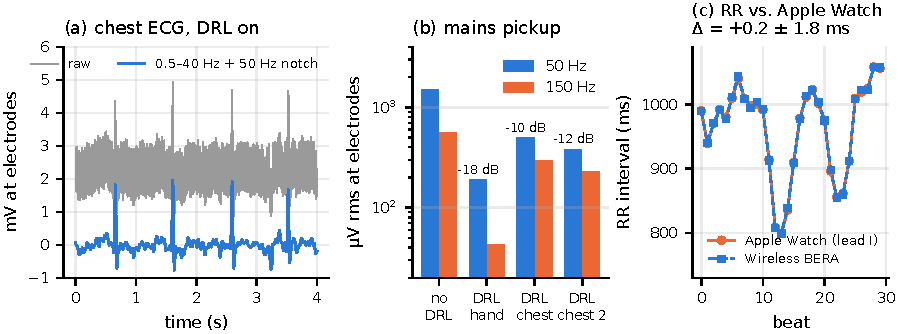
\includegraphics[width=\linewidth]{figures/fig_ecg_drl.pdf}
	\caption{(a) Chest ECG with DRL, raw (offset) and filtered. (b) Mains pickup for the four DRL configurations. (c) Beat-by-beat RR intervals of Wireless BERA and an Apple Watch recorded at the same time.}
	\label{fig:ecg}
\end{figure}
\begin{multicols}{2}

\subsection{Auditory Brainstem Response}
\label{sec:abr}

\paragraph{Setup.} Electrode+ was placed at the high forehead, electrode$-$ on the left mastoid and the DRL on the right mastoid (Figure~\ref{fig:electrode}). Rectangular \SI{105}{\micro\second} clicks were presented to the left ear at \SI{21.1}{\per\second} with alternating polarity. The rate is deliberately not a submultiple of \SI{50}{\hertz}: the mains phase then rotates from sweep to sweep (by \SI{133}{\degree}) and averages out, whereas at \SI{20}{\per\second} or \SI{25}{\per\second} the harmonics would add up coherently. The stream ran at \SI{24}{\kilo\hertz} (\SI{48}{\kilo\hertz} with 2:1 decimation), where about \SI{1.1}{\percent} of packets were lost; at \SI{48}{\kilo\hertz} the Wi-Fi link lost about \SI{11}{\percent}.

\begin{figure}[H]
	\centering
	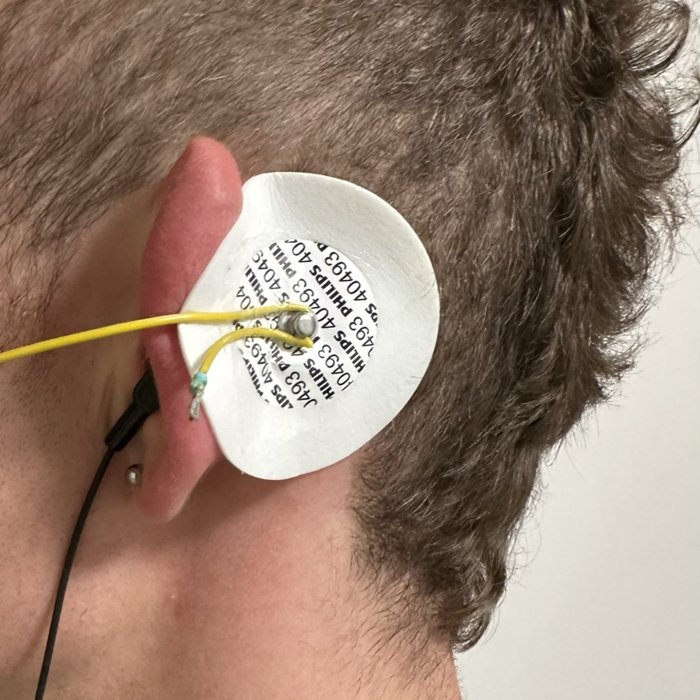
\includegraphics[width=0.62\linewidth]{figures/fig_electrode_mastoid.jpg}
	\caption{Electrode$-$ on the left mastoid. The earbud cable (black) passes right over the electrode; it couples the electrical click artefact into the recording.}
	\label{fig:electrode}
\end{figure}

\paragraph{Processing.} The continuous recording was band-pass filtered (\SIrange{100}{1500}{\hertz}, zero phase) and notch filtered at all \SI{50}{\hertz} harmonics, then cut into sweeps from \SIrange{-2}{12}{\milli\second}. Time zero is the electrical click artefact, found from the alternating-polarity difference. Sweeps above \SI{\pm 25}{\micro\volt} were rejected in $\pm$ pairs, so that artefact and cochlear microphonic keep cancelling, together with restless 64-sweep blocks. Significance was tested by permuting the signs of whole $\pm$ pairs (1000 permutations), which keeps the artefact cancelled but destroys any stimulus-locked response.

\paragraph{Results.} Four runs with six stimulus conditions were recorded (Table~\ref{tab:abr}). Run~2, lying down with click amplitude 0.05 of DAC full scale, shows a significant stimulus-locked response with a positive peak at \SI{6.1}{\milli\second} (bootstrap 95\,\% CI \SIrange{5.8}{6.3}{\milli\second}) and about \SI{160}{\nano\volt} amplitude (Figure~\ref{fig:abr}). Both click polarities show it, so it is neither stimulus artefact nor cochlear microphonic, and its latency fits wave~V at a moderate level. In the control run the earbud was taken out of the ear and placed next to the head, with clicks of similar level (0.035): the electrical artefact remains, the peak at \SI{6}{\milli\second} does not ($p = 0.46$). Run~1 shows the peak at the same latency but stays below significance, as do the runs with fainter clicks and a tone burst.

\begin{table}[H]
	\caption{ABR runs (\SI{21.1}{\per\second}, left ear). Noise: sweep SD range over 64-sweep blocks.}
	\begin{tabular}{L{0.44\linewidth} R{0.13\linewidth} R{0.17\linewidth} R{0.11\linewidth}}
		\toprule
		\textbf{Run} & \textbf{sweeps} & \textbf{noise} & $\boldsymbol{p}$ \\
		& & \si{\micro\volt} & \\
		\midrule
		1 click 0.10, seated & 3904 & 2.9--4.1 & 0.24 \\
		2 click 0.05, lying & 5504 & 1.9--2.2 & \textbf{0.001} \\
		3 click 0.035 & 4416 & 4.7--7.0 & 0.89 \\
		3 sham (no sound) & 3840 & 4.1--5.9 & 0.76 \\
		3 tone burst \SI{2}{\kilo\hertz} & 4224 & 3.2--4.7 & 0.12 \\
		4 earbud out (control) & 4608 & 3.5--5.5 & 0.46 \\
		\bottomrule
	\end{tabular}
	\label{tab:abr}
\end{table}

\end{multicols}
\begin{figure}[H]
	\centering
	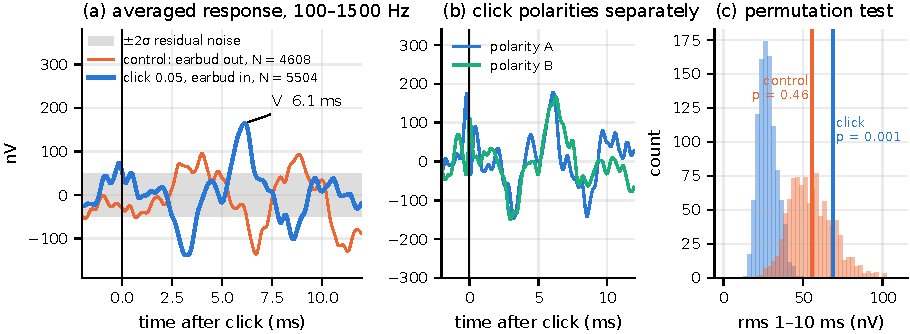
\includegraphics[width=\linewidth]{figures/fig_abr.pdf}
	\caption{(a) Averaged response of run~2 (blue) with wave-V candidate, and of the earbud-out control (orange); grey: $\pm 2\sigma$ of the residual noise of run~2. (b) Run~2 averaged separately for the two click polarities. (c) Permutation null distributions and observed values.}
	\label{fig:abr}
\end{figure}
\begin{multicols}{2}

\subsection{What Limits the Noise}

The noise per sweep, not the electronics, decides whether a run shows a response. Over all runs it follows the EMG power of neck, jaw and forehead muscles closely ($R^2 = 0.86$ on a log scale, Figure~\ref{fig:noise}). In run~2 it fell from \SI{20}{\micro\volt} to \SI{2.2}{\micro\volt} once the subject had settled, after about \SI{130}{\second}. Above \SI{1.5}{\kilo\hertz}, where little biological signal remains, all runs share the same floor of about \SI{32}{\nano\volt\per\sqrt\hertz}, close to the expected amplifier and quantisation noise.

The other interference sources turned out to be negligible:
\begin{itemize}
	\item \textbf{Mains:} \SIrange{0.2}{6}{\micro\volt} at the head with DRL, against \SI{1.5}{\milli\volt} at the chest without; no harmonic is detectable after the notch filters.
	\item \textbf{Wi-Fi:} no artefact at the packet rate or the beacon interval (below \SI{30}{\nano\volt}). The packet losses fall on a fixed \SI{524}{\milli\second} grid of the Wi-Fi link and only cost about \SI{4.5}{\percent} of the sweeps.
	\item \textbf{Heart:} no ECG is detectable at the head (below \SIrange{10}{15}{\micro\volt}); its residual in the average is below \SI{1}{\nano\volt}.
	\item \textbf{Battery:} no change in noise or spurs as the cell fell from \SIrange{3.42}{3.23}{\volt}.
\end{itemize}

\begin{figure}[H]
	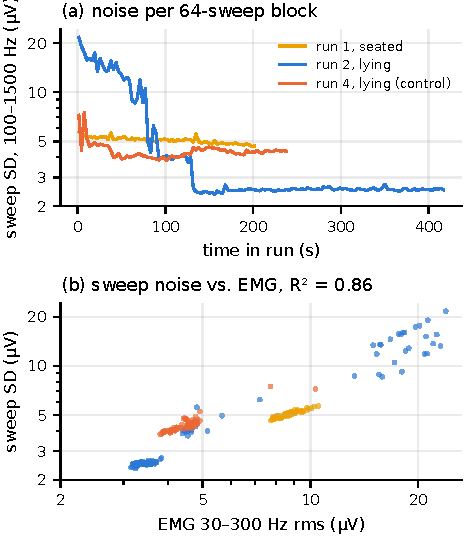
\includegraphics[width=\linewidth]{figures/fig_noise.pdf}
	\caption{(a) Sweep noise over time. (b) Sweep noise against EMG (\SIrange{30}{300}{\hertz}) per 64-sweep block.}
	\label{fig:noise}
\end{figure}

\subsection{Other Signals in the Data}

The same recordings contain more than the ABR. The forehead electrode picks up eye blinks (about \SI{100}{\micro\volt}; 7 per minute seated, 1--2 per minute lying relaxed), and lying down with eyes closed shows a clear alpha rhythm at \SI{10}{\hertz}. The headset microphone shows every click as electrical crosstalk that scales exactly with the click amplitude, and the acoustic click only when the earbud is out of the ear. It can therefore serve as a stimulus monitor and as a check that the earbud is in place.

%-------------------------------------------------------------------------------------
\section{Limitations and Next Steps}

\paragraph{Measurements.} The ABR result rests on one subject, one evening and one significant run. The control run was noisier than run~2 and supports the result rather than proving it. The click level is not calibrated in dB. Next: a level series with interleaved earbud-out controls, a latency--intensity curve and a calibrated click.

\paragraph{Firmware.} The 16-bit stream uses only \SI{1.7}{\percent} of its range at gain~16; 24-bit samples or digital gain before truncation would remove the quantisation contribution. Exact click-onset markers in the packet header, a larger transmit buffer against the periodic Wi-Fi gaps and a live EMG gate that discards restless blocks would make measurements faster and more robust.

\paragraph{Hardware.} For the next revision: a series resistor and clamp in front of the codec inputs (a saturated amplifier on $\pm\SI{5}{\volt}$ can exceed the codec's absolute maximum), I\textsuperscript{2}C pull-ups to the codec supply, the remaining open values of the electrode network, and the charger status routed to the MCU. The earphone cable should be twisted and led away from the electrode leads.

%-------------------------------------------------------------------------------------
\section{Conclusion}

Wireless BERA v1.0 was designed, manufactured, assembled and brought into operation. On battery and over Wi-Fi it records a clean ECG that agrees beat for beat with a commercial device, its driven right leg lowers mains interference by up to \SI{18}{\decibel}, and it recorded a click-evoked brainstem response with a wave-V candidate at \SI{6.1}{\milli\second}. The measurements also show where the remaining limit lies: in the muscle activity of the subject, not in the electronics.

%-------------------------------------------------------------------------------------
\section*{Use of AI Tools}
\addcontentsline{toc}{section}{Use of AI Tools}
This report, the measurement scripts and parts of the firmware were drafted with the AI assistant Claude (Anthropic), working from the project files and the author's instructions; the author reviewed the results. The hardware design, assembly and measurements are the author's own work.

	\end{multicols}

	\begin{multicols}{2}
		\addcontentsline{toc}{section}{References}
		\printbibliography[title=References]
	\end{multicols}

	\newpage
	\vfill % Push text to the bottom of the page
\begingroup
	\footnotesize % Reduce font size
	\subsection*{Disclaimer}
		This report is intended for internal use within the organization only. The information and assessments provided are preliminary and not intended for external distribution. No guarantee is given for the accuracy or completeness of the content. The findings and interpretations reflect the current state of analysis and may be subject to revision. Use of this document for decision-making should be done with appropriate technical review.
	\subsection*{Copyright}
		\textcopyright~\the\year{} Munich Institute of Biomedical Engineering, Technische Universität München 
		
		This document and its contents are protected by copyright. Reproduction, distribution, or use beyond internal purposes is not permitted without prior written consent. All rights reserved. Unauthorized use may result in legal consequences. This document may also contain confidential information; any unauthorized disclosure is strictly prohibited.

	\subsection*{Contact}
		Munich Institute of Biomedical Engineering\\
		Technische Universität München\\
		Boltzmannstrasse 11\\
		85748 Garching\\
\endgroup

\end{document}
